\documentclass{beamer}

\usepackage[utf8]{inputenc}

\usepackage[export]{adjustbox}

\usepackage{listings}
\usepackage{xcolor}
\usepackage{biblatex}
\usepackage{multirow}

\addbibresource{../background/software-diversity/software_diversity.bib}
\addbibresource{../background/llvm/llvm.bib}
\addbibresource{../background/constraint-programming/constraint_programming.bib}
\addbibresource{../background/unison/unison.bib}

\begin{document}

\begin{frame}
	\frametitle{Introduction}

	A Systematic Approach to Automated Software Diversity using Unison

	\vspace{0.5cm}

	Systematically generating diverse executables using a constraint solver is at least as good as basing the diversification process on randomization.

	\begin{enumerate}
		\item Software Diversity
		\item Constraint Programming
		\item Unison
		\item Experiment \& Result
		\item Summary \& Conclusion
	\end{enumerate}

\end{frame}

\section{Software Diversity}

Software diversity is a diverse field, and there is research focusing on different areas
with different goals in mind. However, what they all have in common is the that they are
exploring the potential benefits of engineering diversity within software development.
When talking about software diversity there are a few different classifications and goals
\cite[Section~1]{survey} which will be covered here.

Software diversity has a diverse (heh) set of goals ranging from fault-tolerance to re-usability
to security \cite{survey}.

\subsection{Managed Software diversity}

Managed software diversity is the notion of encouraging or controlling software diversity.

\subsubsection{Natural Diversity}

A lot of software with similar features naturally and spontaneously emerges from engineering
processes. There are a multitude of products from competing organizations that provide
the same function, for example routers, web browsers, compilers, database management systems
and firewalls. Natural diversity could also be something as simple as one program being
tunable by parameters to provide different functionality and performance \cite{survey}.

\subsubsection{Design Diversity}

Design diversity is the process of introducing diversity through the design process. For
example, \textit{N-version programming} is the approach where $N \geq 2$ functionality equivalent
programs are developed from the same specification. The point of this is that hopefully
it will result in a subset of the programs being free from bugs that another subset
might suffer from, thus creating a more fault tolerant system \cite{n-version}.

\subsection{Automated Software Diversity}

\textcite{survey} describes automated software diversity as \say{techniques for artificially
and automatically synthesizing diversity in software} \cite[\pno~8]{survey}. It is also
known as \textit{synthetic diversity} \cite{synthetic-diversity}. \say{Automated} is
referring to the fact that a human is not part of the diversification process, other than
having designed the framework \cite[Section~4]{survey}.

Automated diversity can characterize itself in different ways. A common approach is to
introduce some kind of randomness into software to break the otherwise deterministic behaviour
of most software. This can have several benefits, including security \cite{add-obfuscation}.
Randomization techniques are generally ways to either directly or indirectly create unique
execution of the same program \cite[Section~4.1]{survey}.

\subsubsection{Dynamic Randomization}

By introducing randomization at program run-time one can dynamically diversify the program
and introduce non-deterministic behaviour.

\textcite{os-randomization} randomizes the interface
between user space applications and the operating system by shuffling system call mappings,
changing library entry points and randomizing stack placement.

\textcite{mem-exploits} implements a source-to-source C-code transformer that randomizes
stack-resident variables, static data and individual functions (by introducing a level of
indirection to function calls).

\textcite{binary-stirring} introduces a technique they call \textit{stirring}, where
they accept input in the form of x86 binary code (without debug symbols, source code or
relocation information) and produce a new x86 binary file whose basics block addresses
are stirred and dynamically determined at program load-time.

Of course there are many more techniques and approaches but they will not be covered here.

\subsubsection{Static Randomization}

Static randomization creates diversity at compile time by generating several versions of the
same program that are functionally equivalent but semantically different. This can be done
in a variety of ways including but not limited to: exploiting NOP (no operation) instructions,
instruction set randomization, reversing the stack, stack frame padding,
and obfuscation (register randomization, variable reordering etc)
\cite{survey, compiler-generated-sw-div},

This thesis will focus on static, compiler generated randomization. Just as for dynamic
randomization, static randomization's current focus is security. The key insight is that
while the same source code always yields the same binary in the current climate, the compiler
takes a lot of decisions based on heuristics when reaching this concluding binary (see \ref{sec:llvm}).
It is even the case that those decisions might be flawed and that a different heuristic
might have yielded a better result (see \ref{sec:unison}). Not only does this indicate
that there is room for improvements in present-day compilers, but it also a huge potential
for automated software diversity. For example, if we compile:

\lstinputlisting[label={src:vec-add},caption=A C++ function for adding two vector values,
language=C++,tabsize=2,frame=single,breaklines=true, showstringspaces=false,
backgroundcolor=\color{lightgray}]{background/software-diversity/examples/vec_add.cpp}

we can generate multiple different binaries simply by using multiple different compilers.
Here are two examples using gcc and clang (with -Ofast):

\lstinputlisting[caption=Assembly emitted by gcc for listing \ref{src:vec-add},tabsize=2,
frame=single, breaklines=true,showstringspaces=false,backgroundcolor=\color{lightgray}]
{background/software-diversity/examples/gcc_vec_add.s}

\lstinputlisting[caption=Assembly emitted by clang for listing \ref{src:vec-add},tabsize=2,
frame=single, breaklines=true,showstringspaces=false,backgroundcolor=\color{lightgray}]
{background/software-diversity/examples/clang_vec_add.s}

Even though this function is very small the resulting assembly is very different. In this
case the assembly produced by gcc is basically garbage (in terms of optimizations)
compared to the one produced by clang (a difference of 20 instructions) but nonetheless
they are two functionally equal but semantically different binaries. This is to emphasise
that software diversity is not a foreign concept, but rather very commonly occuring.

There are ways to deploy and steer this inherent diversity. \textcite{compiler-generated-sw-div}
have explored two approaches to this. One where they implement a diversification engine for
an App Store (such as Apple's App Store or Google Play Store) that automatically generates
a unique binary for every download. The other approach is to run multiple variants of the
same program at the same time in parallel and verifying that their behaviour is correct.
Both of these approaches can make use of more or less all previously mentioned diversity
techniques, both dynamic and static.

We will explore the diversity potential in integrated instruction scheduling and register
allocation by using a tool that functions by combinatorial exploration of binary programs
that potentially represents the input source code (\ref{sec:llvm} and \ref{sec:unison}).
In other words, it compiles the code by working out possible binary representations of the
program and then iteratively verifying them to find a solution.

\subsection{Why bother?}
\subsubsection{Return Oriented Programming}
Return oriented programming hijacks the call stack to divert control flow in a program. It
works by overwriting the return address of a function call to execute instruction sequences
outside the intended order. By carefully choosing these sequences (called gadgets) an adversary
can perfor arbitrary operations. \textcite{rop} not only introduced this technique
but also showed that more or less all binaries contain enough of these gadgets to execute
arbitrary code (such as opening a shell).

The attack is mainly about identifying these gadgets, construction a sequence of
gadgets to execute the sought-after code and construction a payload which somehow hijacks
the control flow of the program to execute this sequence of gadgets. If we can somehow
break these gadgets then the payload will be useless. However, as \textcite{rop} showed
it is not practically impossible to break all gadgets. What we can do, however, is diversify
our binaries. By compiling several different binaries who all have different instruction
sequences we break these gadgets, and thus make attacking all versions of our program
a lot more resource heavy. As it stands now by construction a payload on one binary you can
attack all of them. If we diversify, that payload only works on the specific binary it was
constructed for.

\textcite{large-scale-automated} explored two static compiler techniques to break these
gadgets, NOP insertion and randomizing instruction scheduling. While they found that their
techiques worked very well they both rely on randomness. More specifically they insert
NOP randomly in the code and randomize the instruction schedule. Both of these techniques
offers no \textit{guarantees} that the resulting binaries will the diverse enough and they
also introduce some overhead when executing the binaries (albeit small).


%return oriented programming: https://www.informatik.tu-darmstadt.de/fileadmin/user_upload/Group_TRUST/PubsPDF/readactor.pdf
% Show gadgets in previously emitted assembly (vec_add)


\begin{frame}
	\frametitle{Constraint Programming}
	Also called \textit{Combinatorial Optimization}.

	\vspace{1cm}

	A programming paradigm where you are describing the charactersitics of a solution
	rather than the steps needed to reach a solution.
\end{frame}

\begin{frame}
	\frametitle{Solving a Problem in 3 easy steps!}

	\begin{enumerate}
		\item Identifying variables and corresponding domains
		\item Determining Constraints
		\item Choosing a search heuristic
	\end{enumerate}
\end{frame}

\begin{frame}
	\frametitle{Identifying Variables}
	$SEND + MOST = MONEY$
	
	\vspace{0.5cm}
	\noindent
	$S \in \{0, 1, 2, 3, 4, 5, 6, 7, 8, 9\}$ \\
	$E \in \{0, 1, 2, 3, 4, 5, 6, 7, 8, 9\}$ \\
	$N \in \{0, 1, 2, 3, 4, 5, 6, 7, 8, 9\}$ \\
	$D \in \{0, 1, 2, 3, 4, 5, 6, 7, 8, 9\}$ \\
	$M \in \{0, 1, 2, 3, 4, 5, 6, 7, 8, 9\}$ \\
	$O \in \{0, 1, 2, 3, 4, 5, 6, 7, 8, 9\}$ \\
	$T \in \{0, 1, 2, 3, 4, 5, 6, 7, 8, 9\}$ \\
	$Y \in \{0, 1, 2, 3, 4, 5, 6, 7, 8, 9\}$
\end{frame}

\begin{frame}
	\frametitle{Determining Constraints}
	Relationship between variables.

	\begin{tabular}{cccccc}
		& & $1000 * S$ & $100 * E$ & $10 * N$ & $D$ \\
		+ &	& $1000 * M$ & $100 * O$ & $10 * S$ & $T$ \\
		\hline
		& $10000 * M$ & $1000 * O$ & $100 * N$ & $10 * E$ & $Y$
	\end{tabular}

\end{frame}

\begin{frame}
	\frametitle{Choosing a Search Heuristic}
	Search heuristic is a fancy word for "how we want to guess".
	
	\vspace{1cm}

	When we can no longer shrink domains but there are still multiple possibilities we guess.
\end{frame}

\begin{frame}
	\frametitle{Propagating and Searching}
	\begin{columns}
		\begin{column}{0.5\textwidth}
			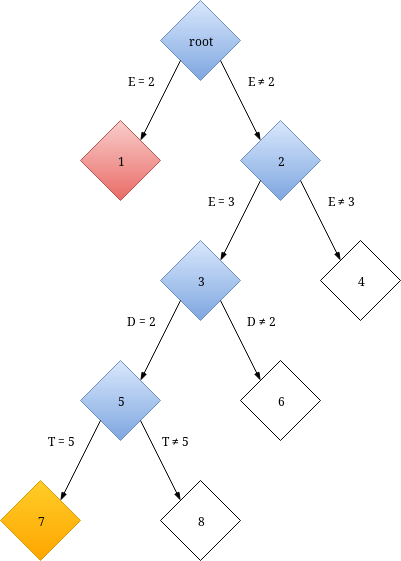
\includegraphics[width=6cm]{../background/constraint-programming/figures/constraint_first_solution}
		\end{column}

		\tabcolsep=0.11cm
		\begin{column}{0.5\textwidth}
			\begin{tabular}{c|c|c|c|c|c}
				Variable & root & 2 & 3 & 5 & 7 \\
				\hline
				S & 9 & 9 & 9 & 9 & 9 \\
				E & 2..7 & 3..7 & 3 & 3 & 3 \\
				N & 3..8 & 4..8 & 4 & 4 & 4 \\
				D & 2..8 & 2..8 & 2,5,6 & 2 & 2 \\
				M & 1 & 1 & 1 & 1 & 1 \\
				O & 0 & 0 & 0 & 0 & 0 \\
				T & 2..8 & 2..8 & 2,5,6 & 5,6 & 5 \\
				Y & 2..8 & 2..8 & 5..8 & 7,8 & 7 \\
			\end{tabular}

		\end{column}
	\end{columns}
\end{frame}

\begin{frame}
	\frametitle{Optimizing}
	Unexplored options

	\vspace{1cm}

	For further combinations to be considered a solution we require $MONEY$ to map to a bigger integer.

	\vspace{1cm}
	
	\centering
	\begin{tabular}{c|c|c|c|c|c|c|c|c}
		S & E & N & D & M & O & T & Y & MONEY \\
		\hline
		9 & 7 & 8 & 2 & 1 & 0 & 4 & 6 & 10876 \\
	\end{tabular}

\end{frame}


\section{Unison}
\label{sec:unison}

Unison is an open-source\footnote{\url{https://github.com/unison-code/unison}},
potentially optimal tool that performs integrated register allocation and instruction
scheduling using constraint programming. It can be used as an alternative or complement to
the algorithms currently in place by compilers such as GCC and LLVM. In particular there
already exists a driver for LLVM which accept input in the form of LLVM MIR \cite{unison-docs}.

\subsection{Constraint Programming}

Constraint programming is a programming paradigm for solving combinatorial problems.
By declaring all variables possible values and their \textit{constraints}, the relationship
between them when part of a solution, a \textit{constraint solver} can search the solution
space and find an assignment of variables to values that is consistent with the constraints.
A constraint solver effectively explores different possible combinations systematically,
by a potentially incomplete local inference (also known as \textit{constraint propagation})
or more commonly a combination of the two \cite{handbook-constraint-programming}.

Currently the only constraint solver supported by Unison is Gecode\footnote{\url{www.gecode.org}}
\cite{unison-docs}, which is a constraint solver that interleaves system search algorithms
search with constraint propagation\cite{MPG}.

When propagating constraints the Gecode solver searches all variable's domains and removes
variables that in conflict with the constraints\cite[Section~23.1]{MPG}. For example,
given two variables (and their corresponding domains) $x \in {0,1,2}$ and $y \in {0,1,2}$
and the constraint $x > y$ constraint propagation can determine that $x \in {1, 2}$ and
$y \in {0, 1}$ are the only combinations consistent with the constraint.

When constraint propagation is finished there are three possible states:

\begin{enumerate}
	\item One or more domains could be empty, proving that no solution exists.
	\item	All domains could be of size 1, indicating that there exists only one possible
		value for every variable, and thus we have found a solution.
	\item One or more variables have multiple values in their domain.
\end{enumerate}

For situation (1) and (2), either a solution is found or we have proven that a solution
does not exist (within the local search space).

In the latter situation (3) the Gecode constraint solver splits a variable's domain into
two or more subsets, creating a \textit{search tree} where each \textit{branch} represents
reducing the variable's domain to a particular subset \cite[Section~8]{MPG}. By commiting
to a branch the constraint solver can once again perform constraint propagation and repeat
the process. However, if \textit{branching} has taken place and the solver reaches
situation (1) it can go back up the tree and explore a different branch. If situation (2)
is reached it can still backtrack but with the added option of adding more constraints
based on the newly found solution. Constraining based on previously found solutions in the
search tree is done with the \textit{branch-and-bound} search engine\cite[Section~9]{MPG}
in Gecode.

\textit{Branch and bound} is an efficient strategy to find the optimal solution to a
combinatorial problem which in essence constitutes comparing potential solutions to the
currently best found solution, choosing the better of the two\cite{BaB}. We will adopt a
similar strategy, but instead of constraining solutions to be better we will require them
to be \textit{different}. In addition, no solutions will be discarded.

\subsection{Unison}


Unison models the problems of register allocation and instruction scheduling as a single
constraint-satisfaction problem and solves them simultaneously \cite{unison-docs,reg-alloc-inst-sched-uni}.

Unison's key properties are that it introduces \textit{optional copies} and
\textit{alternative temporaries} \cite{reg-alloc-inst-sched-uni}. This allows Unison to
support different register allocation decision and perform otherwise unreachable optimizations
\cite{reg-alloc-inst-sched-uni, comb-spill}.


\begin{frame}
	\frametitle{Branch and Bound Strategies for Diversity}

	\begin{enumerate}
		\item Enumerate
			\begin{itemize}
				\item Do nothing when a solution is found
				\item The same combination is never explored twice
			\end{itemize}
		\item Registers
			\begin{itemize}
				\item Disallow the same register allocation
			\end{itemize}
		\item Schedule
			\begin{itemize}
				\item Disallow same schedule
			\end{itemize}
	\end{enumerate}

\end{frame}

\begin{frame}
	\frametitle{Data set}

	Unison test suite; Samples from SPEC2006

	\vspace{0.5cm}

	Simulate linking by placing them in the same order every time

	\vspace{0.5cm}
	
	\begin{itemize}
		\item	Execution time of code generator
		\item	Estimated execution time
		\item	Frequency of surviving gadgets
	\end{itemize}

\end{frame}

\begin{frame}
	\frametitle{Experimental Protocol}

	\begin{enumerate}
		\item For every function generate 1000 versions
		\item Version 0 of every function will make up program 0, version 1 will make up program
			1 and so forth
		\item For every program find all gadgets and its cost
		\item Calculate our metrics
		\item Repeat for all strategies
			\begin{itemize}
				\item Enumerate
				\item Registers
				\item Schedule
			\end{itemize}
		\item Repeat for all sampling rates
			\begin{itemize}
				\item 1
				\item 10
				\item 100
				\item 1000
			\end{itemize}
	\end{enumerate}

\end{frame}


\chapter{Results and Discussion}

In this chapter each metric mentioned in Section \ref{sec:metrics} will be presented in
its own section. An interpretation of the result will also be presented for each
metric, but all general discussion will be in chapter \ref{chapter:discussion}.

\section{Generation Time}

\begin{figure}[h]
	\centering
	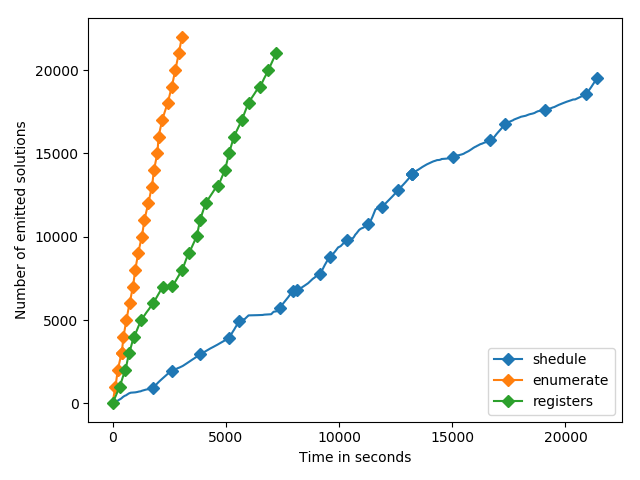
\includegraphics[width=\textwidth,height=0.5\textheight]{results/figures/generator_time}
	\caption{The execution time of the code generator at sampling rate 1000 (i.e 1000000 solutions for every function). Each marker represents the finished generation of a function. The markers are ordered so that the nth marker on every line represents the same function. Total time is annotated as hours and minutes.}
	\label{fig:time}
\end{figure}

The execution times of the constraint solver at sampling rate 1000 are shown in Figure
\ref{fig:time}. Each marker represents the completed generation of a function. That is,
for each marker 1000000 (one million) solutions have been explored. For a few functions
fewer than 1000 solutions were found (for a complete breakdown see appendix
\ref{appendix:function_names}).

While the total execution time is daunting, it does represent about 23 million solutions
found (but only 23000 emitted). The enumerate strategy is fairly quick: 51 minutes for one
million solutions of every function means that on average, one solution was found every
139ns. The same number for registers and schedule is 343ns and 1095ns respectively. To
mitigate the impact of a long execution time the solutions can be emitted directly when
found.

disUnison does not use the same search heuristics as the base Unison model. The disUnison
search heuristics makes implementation easier at the potential cost of execution time. The
problem with optimizing the branching and search heuristics of the model is that the
performance impact will largely have to be determined empirically. Supposedly, the optimal
search heuristic for the registers strategy would not be the same as the optimal search
heuristic for the schedule strategy.

\section{Cost}
\label{sec:cost_result}

\begin{figure}[h]
	\centering
	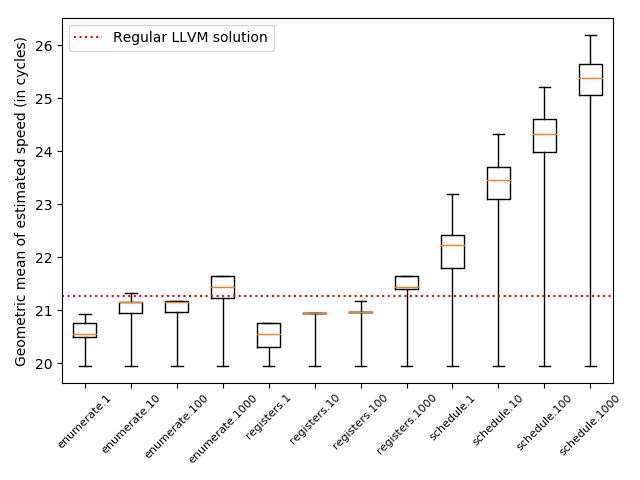
\includegraphics[width=\textwidth,height=0.5\textheight]{results/figures/cost_speed}
	\caption{The cost (speed) distributions for every strategy and sampling rate. The cost of the LLVM solution is included for reference.}
	\label{fig:cost-speed}
\end{figure}

\begin{figure}[h]
	\centering
	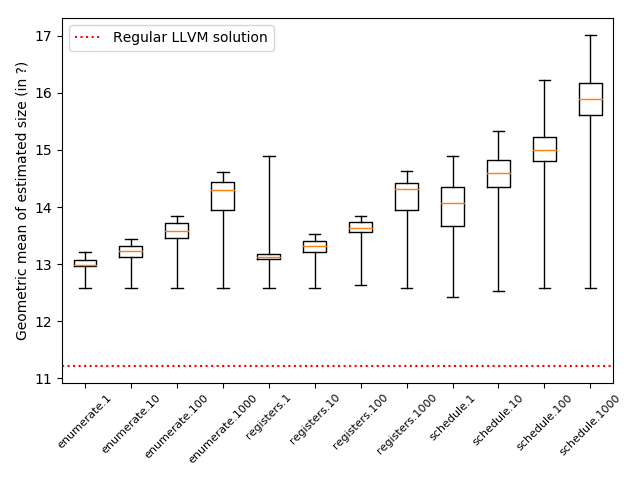
\includegraphics[width=\textwidth,height=0.5\textheight]{results/figures/cost_size}
	\caption{The code size distributions for every strategy and sampling rate. The cost of the LLVM solution is included for reference.}
	\label{fig:cost-size}
\end{figure}

Figure \ref{fig:cost-speed} and Figure \ref{fig:cost-size} shows the distributions of the
estimated cost in cycles and the code size for each strategy and sampling rate
respectively. Both the cost in cycles and the code size for a program version is
calculated as the geometric mean between the cost of the individual functions that make
up the program version. That is, for every strategy and sampling rate there are 1000
values for each cost metric, where each value is a geometric mean between the cost values
of 23 functions.

All strategies perform better for lower sampling rates both in terms of speed and in terms
of code size. As described in section \ref{sec:sampling_rate}, this is expected. Both the
enumerate and registers strategy performs very well compared to the LLVM solution
in terms of speed. The schedule strategy incurs a slight overhead for the lowest sampling
rate and a significant overhead for the three higher sampling rates.

The fact that no solution has a size lower than the LLVM solution can be explained by
referring to the optimization goal used, which was speed. The code size has not been taken
into account during branching and no attempt has been made to optimize it.

Interesting to note is that all strategies and sampling rates have found a solution with
an equally low speed. This is the very first solution found and it is upon this solution
the first strategy related constraints are based. Thanks to the search heuristic, where
lower cost solutions are explored first, this is also the optimal speed.

\section{Surviving Gadgets}

\begin{figure}[htp]
	\centering
	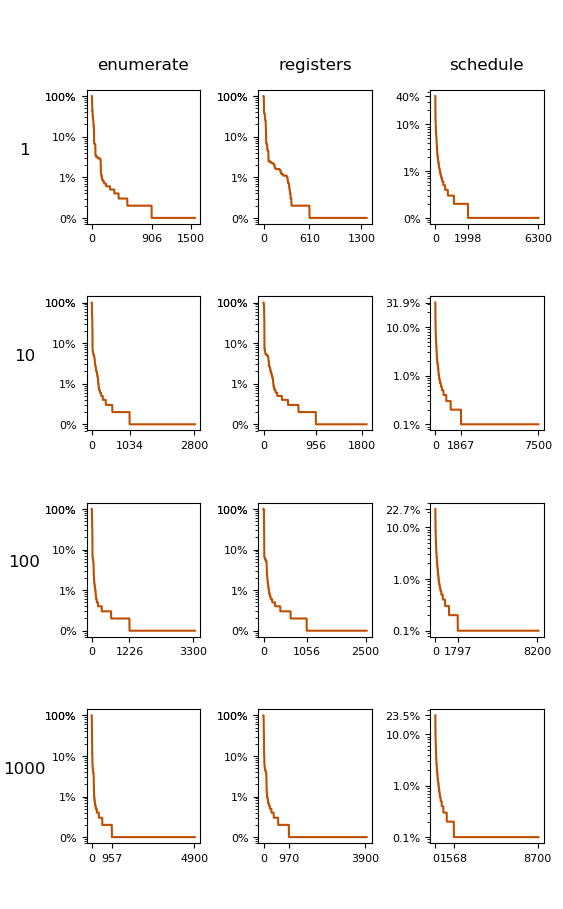
\includegraphics[width=\textwidth,height=\textheight]{results/figures/gadgets}
	\caption{The ratio of occurrence for each gadget broken down by strategy and sampling rate.
The x-axis displays the gadget ids. The first non-zero x-tick and the second non-zero x-tick
displays the first gadget that only appear in one program version and the total number
of unique gadgets, respectively. The data is sorted from most to least frequent to allow
for a better overview.}
	\label{fig:gadgets}
\end{figure}

Figure \ref{fig:gadgets} shows the occurrence ratio of each gadget for the different
strategies and sampling rates. The x-axis shows a gadget id and there is no definitive
correlation between the gadgets across strategies and sampling rates. The ids are ordered
from most frequent to least frequent to better facilitate comparison. The first non-zero
x-tick refers to the id of the first gadget that only appear once and the second non-zero
x-tick is the total number of unique gadgets. E.g the enumerate strategy at sampling rate
1 has $1561-906=655$ gadgets that only appear in one program version. Strategies and
sampling rates that were more effective have a higher number of unique gadgets. The y-axis
is set to a logarithmic scale since the bulk of the data is below 1\%. The frequency of
the most frequent gadget is annotated.

As seen in Figure \ref{fig:gadgets}, neither the enumeration nor the registers strategy
were particularly effective at breaking gadgets for any sampling rate, when compared to
the schedule strategy. There is a slight improvement for higher sampling rates but it is
not particularly impressive even at sampling rate 1000. There are still many gadgets that
survives across a large percentage of versions. The schedule strategy, however, performed
well with no gadget being present in even 50\% of all versions for the lowest sampling
rate and for sampling rate 1000 about 82\% of gadgets only appear in one version.

If an adversary were to construct a payload for a binary from the schedule strategy
at sampling rate 1000 the chances of it working on another binary in that population is
very small. Even if the payload only relies on a single gadget, and that gadget happens
to be the most frequent one, the payload would only work on about 24\% of the binaries. It
is, however, much more likely that an adversary needs multiple gadgets. Since 82\% of
all gadgets are unique to their program version and the gadgets has to be exactly equal on
for the payload to work on another binary it is very unlikely that the adversary can re-use
the payload at all. Unfortunately the schedule strategy also incurred the most overhead,
as seen in Section \ref{sec:cost_result}.

The difference in behavior of the strategies is discussed in Section \ref{sec:discussion}.


\begin{frame}
	\frametitle{Summary and Conclusion}

	Summary
	\begin{itemize}
		\item Code re-use attacks
			\begin{itemize}
				\item Reliant on the arrangement of the executable
			\end{itemize}
		\item Constraint programming \& Unison
		\item The experiments and results
	\end{itemize}

	\vspace{0.5cm}
	
	Conclusion
	\begin{itemize}
		\item Easy to implement
		\item A lot of control of the generated code
		\item Diverse populations
		\item Has to be repeated on a proper executable targeting x86
	\end{itemize}

\end{frame}

\end{document}
